%% these.tex
%% Copyright 2010 Luca De Feo
%% All rights reserved


\section{The algorithm \alg{C2-AS-FI}}
\label{sec:C2-AS-FI}

The most expensive step of \ctwoas{} is the polynomial interpolation step
which is part of the Cauchy interpolation. If we use a standard
interpolation algorithm, its input consists in a list of $\Theta(p^k)$
pairs $\bigl(P, \I(P)\bigr)$, with $P$ having coordinates in $\U_k$,
thus a lower bound for any such algorithm is $\Omega(p^{2k}d)$. Notice
however that the output is a polynomial of degree $\Theta(p^k)$ in
$\F_q[X]$, hence, if supplied with a shorter input, an \emph{ad hoc}
algorithm could reach the bound $\Omega(p^kd)$.

In this section we give an algorithm that reaches this bound up to
some logarithmic factors. It realizes the polynomial interpolation on
the primitive points of $E[p^k]$, thus its output is a degree
$\euler(p^k)/2-1$ polynomial in $\F_q[X]$. Using the
\titleref{th:chinese-remainder} it is straightforward to generalize
this to an algorithm, having the same asymptotic complexity, that
realizes the polynomial interpolation on all the points of
$E[p^k]$. We call \ctwoasfi{} (FI for Fast Interpolation) the variant of
\ctwoas{} resulting from applying this new algorithm.


\subsection{The algorithm}
Let $P\in E[p^k]$ and $P'\in E'[p^k]$ be primitive $p^k$ torsion
points. We want to compute the polynomial $A\in\F_q[X]$ such that
\begin{equation}
  A\bigl(x\bigl([n]P\bigr)\bigr) = x\bigl([n]P'\bigr)
  \quad\text{for any $n\in\left(\Z/p^k\Z\right)^\ast$.}
\end{equation}
As we saw in Section~\ref{sec:chin-rema-algor}, such a polynomial is
only defined modulo the polynomial vanishing on the interpolation
points
\begin{equation}
  T(X) = \prod_{n\in\left(\Z/p^k\Z\right)^\ast} \bigl(X - x([n]P)\bigr)
  \text{.}
\end{equation}
Thus we look for the canonical representative of $A$ in $\F_q[X]/T(X)$.

We start by applying the \titleref{th:chinese-remainder} to
$\F_q[X]/T(X)$: let
\begin{equation}
  \label{eq:T}
  T = \prod T^{(j)}
\end{equation}
be the factorization of $T$ over $\U_0$, and set
\begin{equation}
  \label{eq:A}
  A^{(j)} \eqdef A \bmod T^{(j)}
  \;\text{.}
\end{equation}
Define
\begin{equation}
  \label{eq:187}
  \K_j\eqdef\F_q[X]/T^{(j)}(X)  
  \text{,}
\end{equation}
then $\K_j$ is a field and $A^{(j)}$ is the projection of $A$ in
$\K_j$.

It was already pointed out in~\cite[$\S$2.3]{couveignes96} that,
knowing the factorization of $T$ over $\U_0$ and all the $A^{(j)}$'s,
we can recover $A$ using the Chinese remainder algorithm
of~\cite[$\S10$]{vzGG} (see also
Section~\ref{th:chinese-remainder}). Thus we will focus on computing,
say, $A^{(0)}$.

Choose any root $\zeta$ of $T^{(0)}$, without loss of generality we
can take $\zeta=x(P)$, then
\begin{equation}
  \label{eq:188}
  \basis{B}=\{1,\zeta,\ldots,\zeta^{d-1}\}  
\end{equation}
is an $\F_q$-basis of $\K_0$.  Fix the $\F_q$-linear embedding of
finite fields
\begin{equation}
  \label{eq:embed}
  \xymatrix{
    \K_0 \ar@{^{(}->}[r]^-\iota & \U_k
  }
\end{equation}
given by $\iota(\zeta) = x(P)$, by linearity it is evident that
\begin{equation}
  \iota\bigl(A^{(0)}(\zeta)\bigr) = A^{(0)}\left(\iota(\zeta)\right)=x\bigl(P'\bigr)
  \text{.}
\end{equation}
Thus $\iota^{-1}\bigl(x(P')\bigr)$ is in $\K_0$ and the coefficients
of $A_0$ are its coordinates in the basis $\basis{B}$. In conclusion,
computing $A_0$ is equivalent to find a \hyperref[eq:22]{rational
  univariate representation} of $x(P')$ with respect to $x(P)$.

Unfortunately, applying algorithm \titleref{alg:rur} is not optimal: the
bottleneck is the power projection $\proj_\zeta$ appearing in
step~\ref{alg:rur:1}. We have seen in
Section~\ref{sec:shoups-algorithm} that the dual problem to power
projection is polynomial evaluation, thus in particular
\begin{equation}
  \label{eq:189}
  \begin{aligned}
    \dual{\proj_\zeta} = \ev_\zeta : \F_q[X] &\ra \K_j\text{,}\\
    g &\mapsto g(\zeta)\text{;}
  \end{aligned}
\end{equation}
so that any algorithm to evaluate polynomials at $\zeta$ yields a
power projection algorithm having the same complexity, and
\emph{vice-versa}. But none of the algorithms of
Chapter~\ref{cha:artin-schr-towers} allows to evaluate polynomials in
$\F_q[X]$ at a generic point of $\U_k$, better than a Horner rule.

We shall thus give an alternative algorithm to compute the minimal
polynomial $T_0$ of $x(P)$. It will be similar to a
\hyperref[sec:chin-rema-algor]{subproduct tree}, but it will exploit
the structure of the Artin-Schreier tower. This is similar to the way
we solved Artin-Schreier equations in
Section~\ref{sec:couveignes-algorithm}.


\paragraph{Interpolation in towers of extensions}
We set $\U_0=\F_q$. The algorithm we give here can be applied in any
tower of cyclic extensions, provided the action of the Galois groups
can be computed. However we will present it only for our specific
tower $(\U_0,\dots,\U_k)$, to avoid adding unnecessary notation.

Consider the following problem: given elements $x,y\in\U_k$ such that
$x$ generates $\U_k$ over $\F_q$, find a polynomial $A\in\F_q[X]$ such
that
\begin{equation}
  \label{eq:affine-minimal}
  A(x) = y
  \text{.}
\end{equation}
Let $T$ be the minimal polynomial of $x$ over $\F_q$, then, as above,
the class of $A$ in $\F_q[X]/T(X)$ is uniquely determined.

Let $A$ be a polynomial satisfying \eqref{eq:affine-minimal} it is
clear that $A(\sigma(x)) = \sigma(y)$ for any
$\sigma\in\Gal(\U_k/\F_q)$. Conversely, the polynomial interpolating
$\sigma(x)$ over $\sigma(y)$ for any $\sigma$ is invariant under
$\Gal(\U_k/\F_q)$, thus it has coefficients in $\F_q$. Hence we can
construct $A$ by interpolation.

A \hyperref[sec:chin-rema-algor]{fast interpolation algorithm} would
compute $T$ via a binary subproduct tree, and then interpolate $A$
recursively applying the \titleref{th:chinese-remainder} along the
branches of the tree. However this is too expensive. We can do better
by using a non-binary subproduct tree on which the tower of Galois
groups associated to $(\U_0,\ldots,\U_k)$ acts.

First we need to compute $T$. Let $T_i$ be the minimal polynomial of
$x$ over $\U_i$, we compute it recursively as
\begin{align}
  T_k &= (X - x)\text{,}\\
  \label{eq:minprod}
  T_{i-1} &= \prod_{\sigma\in\Gal(\U_{i}/\U_{i-1})}T_{i}^\sigma\text{.}
\end{align}
Then $T=T_0$. Observe that, rather than computing a whole subproduct
tree of $T$, we have only computed one branching as shown in figure
\ref{fig:tree}.

\begin{figure}[tb]
  \centering
  
  \begin{tikzpicture}
    \begin{scope}
      [level distance=1cm]
      \node{$\U_0$}[grow'=up]
      child {node {$\U_1$}
        child {node {$\U_2$}
          child {node {$\U_3$}}
        }
      };
    \end{scope}    
  \end{tikzpicture}
  % 
  \hfill
  %
  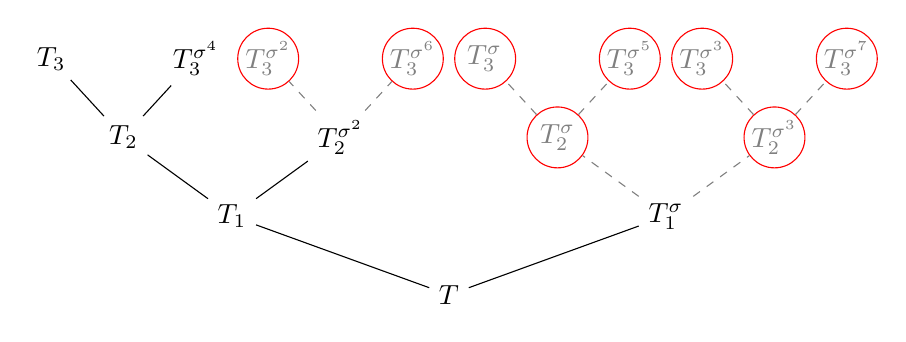
\begin{tikzpicture}
    \begin{scope}
      [level distance=1cm,
      level/.style={sibling distance=\textwidth/(2.2*#1)},
      nc/.style={gray,nodes={circle,draw=red,solid,inner sep=0pt,minimum size=22pt}}]
      \node{$T$}[grow'=up]
      child {node {$T_1$}
        child {node {$T_2$}
          child {node {$T_3$}}
          child {node {$T_3^{\sigma^4}$}}
        }
        child {node {$T_2^{\sigma^2}$}
          child[nc] foreach \l in {2,6} {node {$T_3^{\sigma^{\l}}$} edge from parent[dashed]}
        }
      }
      child {node {$T_1^\sigma$}
        child[nc] {node {$T_2^\sigma$} edge from parent[dashed]
          child[nc] foreach \l in {,5} {node {$T_3^{\sigma^{\l}}$} edge from parent[dashed]}
        }
        child[nc] {node {$T_2^{\sigma^3}$} edge from parent[dashed]
          child[nc] foreach \l in {3,7} {node {$T_3^{\sigma^{\l}}$} edge from parent[dashed]}
        }
      };
    \end{scope}
  \end{tikzpicture}
  
  \pdfmctwo{Circled nodes.}
  \caption{The subproduct tree of $T$, in the case of a tower of
    quadratic extensions. Any generator of $\Gal(\U_3/\U_0)$ can be
    taken as $\sigma$. We gray out and circle the nodes that the
    algorithm does not compute.}
  \label{fig:tree}
\end{figure}


Now the we have something like a subproduct tree for $T$, we proceed
as for interpolation. We compute recursively the polynomials in
$A_i\in\U_i[X]$ such that $A_i(x)=y$. We start from $A_k=y$. Suppose
$A_{i+1}$ is known, then we use the \titleref{th:chinese-remainder} to
obtain the polynomial $P\in\U_{i+1}[X]/T_i(X)$ such that
\begin{equation}
  \label{eq:crt}
  P \equiv A_{i+1}^\sigma \bmod T_{i+1}^\sigma
  \qquad\text{for any $\sigma\in\Gal(\U_{i+1}/\U_i)$.}
\end{equation}
It is clear that $P$ is invariant under $\Gal(\U_{i+1}/\U_i)$, hence
$P\in\U_i[X]/T_i(X)$ and by \eqref{eq:crt} it is evident that
$P(x)=A_{i+1}(x)=y$, thus $P=A_i$.

\pdfmctwo{Éric asked for the difference between Enge-Morain and this
  section. There is none in the algorithm, so I must at least say
  something about what is new in this section. Btw, the "Hecke
  representation" is just an instance of rational univariate
  representation.} We have thus succeeded in interpolating $A=A_0$,
without having to build the whole subproduct tree. A similar algorithm
was applied by Enge and Morain to the solution of equations by
radicals~\cite{enge+morain03}, although they did not recognize the
application to polynomial interpolation.

\begin{remark}
  Observe that, once the polynomials $T_i$ for $0\le i\le k$ are
  known, we have an efficient algorithm to evaluate polynomials in
  $g\in\U_0[X]$ at the point $x$: simply compute
  \begin{equation}
    \label{eq:191}
    \begin{aligned}
      g_0 &= g\bmod T_0\text{,}\\
      g_1 &= g_0\bmod T_1\text{,}\\
      \vdots\\
      g_k &= g_{k-1}\bmod T_k\text{,}\\
    \end{aligned}
  \end{equation}
  then $g_k=g(x)$. Transposing this algorithm gives a power projection
  algorithm that can be used in \titleref{alg:rur}. By the discussion in
  Section~\ref{sec:transp-eucl-divis}, the
  \index{transposed~modular~reduction}transpose of this algorithm
  amounts to iteratively extend a linearly recurring
  sequence. However, we do not use this method because it would not
  improve the overall complexity, as we shall show in the next
  section.
\end{remark}


\paragraph{Back to our problem}
It is easy to realize that, on inputs $x(P)$ and $x(P')$, the
algorithm we just gave computes $A^{(0)}$. In fact, $T^{(0)}$ is
the minimal polynomial of $x(P)$ over $\F_q$ and $A^{(0)}$ is the
unique polynomial in $\F_q[X]/T^{(0)}(X)$ that satisfies
\eqref{eq:affine-minimal}.

This can be viewed as decomposing the morphism $\iota$ of
Eq.~\eqref{eq:embed} as the chain of $\F_q$-linear isomorphisms
\begin{equation}
  \xymatrix{
    ^{\U_0[X_0]}/_{T_0(X_0)} \ar@{^{(}->}[r]^-{\iota_0} &
    \;\cdots\; \ar@{^{(}->}[r]^-{\iota_{k-1}} &
    ^{\U_k[X_k]}/_{T_k(X_k)} \ar@{^{(}->}[r]^-{\iota_k} &
    \U_k
  }
\end{equation}
defined by $\iota_k\circ\cdots\circ\iota_i(X_i) = x(P)$ for any $i$,
and then finding the preimage of $x(P')$ by inverting them one by
one.

Then, the Chinese remainder theorem we applied in \eqref{eq:crt}
amounts to invert $\iota_i$ by descending the lower path in the
diagram below
\begin{equation}
  \xymatrix{
    ^{\U_i[X_i]}/_{T_i(X_i)} \ar@{^{(}->}[r]^-{\iota_i} \ar@{^{(}->}[d]^{\varepsilon} &
    ^{\U_{i+1}[X_{i+1}]}/_{T_{i+1}(X_{i+1})} \\
    ^{\U_{i+1}[Y]}/_{T_i(Y)} \ar@{^{(}->>}[r]^-{\gamma} &
    \bigoplus_\sigma {}^{\U_{i+1}[Y_{j}]}/_{\left(T_{i+1}\right)^\sigma(Y_{j})} \ar@{->>}[u]_{\pi}
  }
\end{equation}
where $\varepsilon$ is the canonical injection extending
$\U_i\subset\U_{i+1}$, $\gamma$ is the Chinese remainder isomorphism
and $\pi$ is projection onto the first coordinate.

Some care must be taken when $x(P)$ does not generate $\U_k$, but only
a subfield of index $2$. This happens when $c\not\in\F_q[c^2]$, and in
this case $\iota_0$ is not a field isomorphism. It is not to
difficult, however, to handle this case, as one only needs to take a
subgroup of index $2$ of $\Gal(\U_1/\U_0)$, instead of the whole
group, in the interpolation algorithm given above.


\subsection{Complexity analysis}
\label{sec:C2-AS-FI:complexity}

In practice, the algorithms to compute $T^{(0)}$ and $A^{(0)}$ are
modified versions of the subproduct tree and the interpolation (see
Section~\ref{sec:chin-rema-algor}).

We set some notation. Let $i_0$ be the largest index such that
$\U_{i_0} = \U_1$ and let $\frac{p-1}{2r} = [\F_q[c^2]:\F_q]$.  Note
that all the $T^{(j)}$'s have degree $\frac{\euler(p^{k-i_0+1})}{2r}$.

We first compute the \emph{truncated} subproduct tree as in
Figure~\ref{fig:tree}. The product of Eq.~\eqref{eq:minprod} is
computed via a classic binary subproduct tree to keep the complexity
low.

\begin{algorithm}
  \caption{Truncated subproduct tree}
  \begin{algorithmic}[1]
    \REQUIRE $x(P)\wrt\U_k$.
    \ENSURE The subproduct tree.
    \STATE Let $T_k = (X - x(P))$;
    \FOR {$i=k-1$ \TO $0$}
    \FORALL {$\sigma \in \Gal(\U_{i+1}/\U_i)$}
    \STATE\label{alg:T:gal} compute $T_{i+1}^\sigma$  using \titleref{alg:iterfrobenius};
    \ENDFOR
    \STATE\label{alg:T:prod}  $T_i\la\prod_\sigma T_{i+1}^\sigma$ 
    via a binary \hyperref[sec:chin-rema-algor]{subproduct tree}.
    \STATE\label{alg:T:push} convert $T_i$  into an element of
    $\U_i[X]$ using \titleref{alg:push-down}.
    \ENDFOR
  \end{algorithmic}
\end{algorithm}

Recall that we denote by $\Lift(i)$ the cost of performing one lift-up
or push-down at the $i$-th level (see Theorem~\ref{theo:L}). For any
$i>i_0$, step~\ref{alg:T:gal} of is repeated $p$ times, each iteration
taking 
\[O\bigl(p^{k-i}\Lift(i-i_0)\bigr) \subset O\bigl(\Lift(k-i_0)\bigr)\]
by Theorem~\ref{th:b-ifrob}.  Step~\ref{alg:T:prod} takes
$O\bigl(\Mult(p^{k-i_0+1}d/r)\log p\bigr)$ using
Algorithm~\ref{alg:subprod} and step~\ref{alg:T:push} takes
\[O\bigl(p^{k-i+1}\Lift(i-i_0)\bigr) \subset
O\bigl(p\Lift(k-i_0)\bigr)\text{.}\]

For any $1\le i<i_0$, there is nothing to do because
$\U_{i+1}=\U_i$. Finally, when $i=0$ and $\U_1\ne\F_q$ the algorithm
is identical but step \ref{alg:T:gal} must be computed through a
generic Frobenius algorithm (using the algorithm of
Section~\ref{sec:modular-composition}, for example) and step
\ref{alg:T:push} must use the implementation of $F_q[c]$ to make the
conversion (for example, linear algebra). In this case
step~\ref{alg:T:gal} costs
$\Theta\bigl(\frac{p^{k-i_0}}{r}\ModComp(pd)\log d \bigr)$
by Eq.~\eqref{eq:204} and step \ref{alg:T:push} costs
$\Theta\bigl(p^{k-i_0}(pd)^2\bigr)$.

Now, we have $T_0$ at the root of the tree. We compute its derivative
$T_0'$ and we evaluate it at $x(P)$ by reducing modulo
$T_1,\ldots,T_k$. This costs strictly less than computing the
subproduct tree.  We finally do the interpolation of $A_0$.

\begin{algorithm}
  \caption{Truncated fast interpolation}
  \begin{algorithmic}[1]
    \REQUIRE $T_i\wrt\U_i[X]$ for $0\le i\le k$, $x(P')\wrt\U_k$, $T_0'(x(P))\wrt\U_k$.
    \ENSURE $A_0\wrt\U_0[X]$.
    \STATE\label{alg:A}  $P_k \la x(P')/T_0'(x(P))$;
    \FOR {$i = k-1$ \TO $0$}
    \FORALL {$\sigma \in \Gal(\U_{i+1}/\U_i)$}
    \STATE\label{alg:A:gal} compute $P_{i+1}^\sigma$ using \titleref{alg:iterfrobenius};
    \ENDFOR
    \STATE\label{alg:T:lift} convert $T_i$ into an element of $\U_{i+1}[X]$ using \titleref{alg:liftup}.
    \STATE\label{alg:A:CRA} $P_i\la \sum_{\sigma}P_{i+1}^\sigma T_i/T_{i+1}^\sigma$ using the binary subproduct tree computed previously;
    \STATE\label{alg:A:push} convert  $P_i$ into an element of
    $\U_i[X]$ using \titleref{alg:push-down}.
    \ENDFOR
    \STATE return $P_0$.
  \end{algorithmic}
\end{algorithm}

Step~\ref{alg:A} is just one inversion in $\U_k$, that is
$O(\Mult(p^{k-i_0}d/r)\log p^{k-i_0}d/r)$. Steps~\ref{alg:A:gal}
and~\ref{alg:A:push} are identical to steps~\ref{alg:T:gal}
and~\ref{alg:T:push} of the subproduct tree and step~\ref{alg:T:lift}
is also absorbed. Finally, step~\ref{alg:A:CRA} has the same
complexity as step~\ref{alg:T:prod} of the subproduct tree, using the
Algorithm~\ref{alg:interp}.

In conclusion, the total cost of computing the subproduct tree and the
interpolation is
\ifafourps
\begin{equation*}
  O\biggl(\bigl(k-i_0\bigr)p\Lift(k-i_0) + \Mult\left(\frac{p^{k-i_0+1}d}{r}\right)\log \frac{p^{k-i_0}d}{r} +
  \frac{p^{k-i_0}}{r}\bigl(\ModComp(pd)\log d + r(pd)^2\bigr)\biggr)
  \text{.}
\end{equation*}
\else
\begin{multline*}
  O\biggl(\bigl(k-i_0\bigr)p\Lift(k-i_0) + \Mult\left(\frac{p^{k-i_0+1}d}{r}\right)\log \frac{p^{k-i_0}d}{r} +\\
  \frac{p^{k-i_0}}{r}\bigl(\ModComp(pd)\log d + r(pd)^2\bigr)\biggr)
  \text{.}
\end{multline*}
\fi

\paragraph{The complete interpolation}
We compute all the $A^{(j)}$'s using this algorithm; there are
$p^{i_0-1}r$ of them. We then recombine them through a
\hyperref[sec:chin-rema-algor]{Chinese remainder algorithm} at a cost
of $O\bigl(\Mult(p^kd)\log p^kd\bigr)$. The total cost of the whole
interpolation phase is then
\begin{equation*}
  O\left(\bigl(k-i_0\bigr) p\Lift(k) + p^{k-1}\ModComp(pd)\log d +
    p^{k-1}r(pd)^2 + \Mult(p^kd)\log p^kd \right)\text{,}
\end{equation*}
that is
\begin{equation}
  \label{eq:interp}
  O\left(p\Lift(k)\log\left(\frac{\ell}{p^{i_0}}\right) + 
    \Mult(\ell d)\log\ell d +
    \frac{\ell}{p}\ModComp(pd)\log d +
    \ell (pd)^2
  \right)\text{.}
\end{equation}

Alternatively, once $A^{(0)}$ is known, one could compute the other
$A^{(j)}$'s using modular composition with the multiplication maps of
$E$ and $E'$ as suggested in~\cite{couveignes96}. However this
approach does not give a better asymptotic complexity because in the
worst case $A^{(0)}=A$. From a practical point of view, though,
Brent's and Kung's algorithm for modular
composition~\cite{brent+kung}, despite having a worse asymptotic
complexity, could perform faster for some set of parameters. We will
discuss this matter in Section~\ref{sec:C2-AS-FI-MC}.

If more than $\euler(p^k)/2$ points are needed, but less than
$\frac{p-1}{2}$, one can use the previous algorithm to interpolate
over the primitive $p^i$-torsion points for each $i=1,\ldots,k$. The
interpolating polynomials can then be recombined through a
\hyperref[sec:chin-rema-algor]{Chinese remainder algorithm} at a cost
of $O\bigl(\Mult(p^kd)\log p^k\bigr)$, which does not change the
overall complexity of \ctwoasfi{}.


Putting together the complexity estimates of \ctwoas{} and \ctwoasfi{}, we
have the following theorem.

\begin{theorem}
  \label{th:complexity}
  Assuming $\Mult(n) = n\log n\loglog n$, the algorithm \ctwoasfi{} has
  worst case complexity
  \ifafive
  \begin{multline*}
    \tildO_{p,d,\log\ell}
    \left(
      p^2d^3 +
      \ModComp(p)pd +
      (pd)^\omega\log^2\ell +
      p^3\ell^2 d\log^3\ell + \right.\\
      \left. p^2\ell^2 d^2+
      \left(\frac{\ell^2}{p} + p\right)\ModComp(pd)
    \right)
    \text{.}
  \end{multline*}
  \else
  \begin{equation*}
    \tildO_{p,d,\log\ell}
    \ifbfive\!\fi
    \left(
      \ifbfive\!\fi
      p^2d^3 +
      \ModComp(p)pd +
      (pd)^\omega\log^2\ell +
      p^3\ell^2 d\log^3\ell + 
      p^2\ell^2 d^2+
      \left(\ifbfive\!\fi\frac{\ell^2}{p} + p\ifbfive\!\fi\right)\ModComp(pd)
      \ifbfive\!\fi
    \right)
    \ifbfive\!\fi
    \text{.}
  \end{equation*}
  \fi
\end{theorem}



% Local Variables:
% mode:flyspell
% ispell-local-dictionary:"american"
% mode:TeX-PDF
% TeX-master: "../these"
% mode:reftex
% End:
%
% LocalWords:  Schreier Artin pseudotrace Frobenius bivariate Joux Sirvent FFT
% LocalWords:  Couveignes isogenies Schoof isogeny cryptosystems Lercier moduli
% LocalWords:  precomputation arithmetics polylogarithmic Karatsuba embeddings
% LocalWords:  irreducibility
